\section{Erweiterung dynamischer Nash-Flüsse}\label{sec-thin-flows}

Der Abschnitt beginnt mit der Einführung einer neuen Klasse statischer $s$-$t$-Flüsse:

\begin{definition}[Schmaler Fluss mit Zurücksetzen]\label{def-thin-flow}
	Seien ein statischer $s$-$t$-Fluss $x'$ mit Wert $F$ in einem azyklischen Netzwerk $(G, u, s, t)$ mit Ursprung $s$ und Versorgungsrate $d$ sowie eine Teilmenge $E_1\subseteq E$ der Kanten gegeben.
	Der Fluss $x'$ heißt \emph{schmaler Fluss mit Zurücksetzen auf $E_1$}, falls eine Knotenbewertung $l'\in\R^V_{\geq 0}$ existiert, die die folgenden Bedingungen erfüllt:
	\begin{enumerate}[label=(T\arabic*)]
		\item\label{def-thin-flow-source} $l_s' = F/d$,
		\item\label{def-thin-flow-x-zero} $l_w' \leq l_v'$, \tabto{4cm} für $vw\in E \setminus E_1$ mit $x'_{vw}=0$,
		\item\label{def-thin-flow-x-positive} $l_w' = \max(l_v', x'_{vw} / u_{vw} )$,  \tabto{4cm} für $vw\in E\setminus E_1$ mit $x'_{vw} > 0$,
		\item\label{def-thin-flow-resetting-edge} $l_w' = x'_{vw} / u_{vw}$,  \tabto{4cm} für $vw\in E_1$,
		\item\label{def-thin-flow-no-resetting-edge} $l_w' \geq \min_{vw\in \delta^-(w)} l_v'$, \tabto{4cm} falls $\delta^-(w)\cap E_1 = \emptyset$.
	\end{enumerate}
	Der Fluss $x'$ heißt \emph{normiert}, falls $F=d$ gilt.
	Die \emph{Auslastung durch eine Kante $e\in E$ bei \todo{Ausgangsauslastung} $l_v'$ und Flusswert $x_e'$} sei gegeben durch
	$$\rho_e(l_v', x_e'):=\begin{cases}
		\max\{ l_v', x_e' / u_e \}, & \text{falls $e\notin E_1$,}\\
		x_e' / u_e, & \text{falls $e\in E_1$.}
	\end{cases}$$
\end{definition}

\todo{
Dabei nennt man $x_e'/u_e$ die Auslastung einer Kante $e\in E$ i $s$.
Ist $E_1 = \emptyset$, dann ist die Knotenbeschriftung $l_v'$ gerade die Auslastung $\max_{e\in P} x_e'/u_e$ eines jeden $s$-$v$-Pfades $P$ mit positiven Fluss.
Kanten in $E_1$ setzen dann die Auslastung jedes vorangegangenen Pfades auf ihre eigene zurück.
}

\begin{remark}\label{remark-thin-flow}
Hier ist, wie in~\cite[Definition~4]{Cominetti2011}, im Vergleich zu~\cite[Definition~6]{Koch2011} die Bedingung~\ref{def-thin-flow-no-resetting-edge} zusätzlich eingeführt worden.
Diese ist nötig, um im Beweis von Theorem~\ref{thm-alpha-extension-is-nash-flow} zu zeigen, dass die erweiterten Ankunftszeiten tatsächlich mit den angegebenen übereinstimmen.
Ohne diese Bedingung würde dies nämlich nicht gelten, wie man in Abbildung~\ref{figure-labels} erkennen kann.
\end{remark}

\begin{lemma}\label{lemma-thin-flow-node-labels}
	Für jeden $F$-wertigen $s$-$t$-Fluss $x'$ in einem azyklischen Netzwerk $(G, u, s, t)$ mit Ursprung $s$ und Versorgungsrate $d$ sowie $E_1\subseteq E$ existiert eine eindeutige Lösung $(l_v')_{v\in V}$ des Gleichungssystems
	$$l_w' = \begin{cases}
		F/d, & \text{falls $w=s$,}\\
		\min_{vw\in \delta^-(w)} \rho_{vw}(l_v', x_{vw}'), & \text{sonst.}
	\end{cases}$$
	Ist $x'$ ein schmaler Fluss mit Zurücksetzen auf $E_1$, so stimmt die zugehörige Knotenbewertung mit der Lösung dieses Systems überein.
\end{lemma}
\begin{proof}
	Die eindeutige Existenz folgt aus der Azyklizität des Graphen.
	Sei $x'$ nun schmaler Fluss mit Zurücksetzen auf $E_1$.
	Man verwende eine Induktion über die Distanz eines Knotens $w$ zu $s$ in $E$ bezüglich der Kantenzahl.
	Für $w=s$ gilt $l_s'=F/d$ bereits nach~\ref{def-thin-flow-source}.
	Für $w\neq s$ ist $l_w'$ nach~\ref{def-thin-flow-x-zero},~\ref{def-thin-flow-x-positive} und~\ref{def-thin-flow-resetting-edge} eine untere Schranke an $\rho_{vw}(l_v', x_{vw}')$ für $vw\in\delta^-(w)$.
	Es bleibt zu zeigen, dass die Auslastung durch eine eingehende Kante gerade $l_w'$ ist:
	Falls eine eingehende Kante in $E_1$ oder eine eingehende Kante mit $x_e'> 0$ existiert, ist die Auslastung durch die Kante $l_w'$ nach~\ref{def-thin-flow-resetting-edge} und~\ref{def-thin-flow-x-positive}.
	Sonst ist $l_w'\geq \min_{vw\in \delta^-(w)} l_v' = \min_{vw\in \delta^-(w)} \rho_{vw}(l_v', x_{vw}')$ nach~\ref{def-thin-flow-no-resetting-edge}, was die Behauptung zeigt.
\end{proof}

\begin{lemma}
	Ein $F$-wertiger statischer $s$-$t$-Fluss $x'$ ist genau dann ein schmaler Fluss mit Zurücksetzen auf $E_1$, wenn $x_{vw}'= 0$ für alle $vw\in E$ mit $l_w' < \rho_{vw}(l_v', x_{vw}')$ gilt.
	Dabei sei $(l_v')_{v\in V}$ die Lösung des Gleichungssystems aus Lemma~\ref{lemma-thin-flow-node-labels}.
\end{lemma}
\begin{proof}
	Angenommen, $x'$ sei ein schmaler Fluss mit Zurücksetzen auf $E_1$.
	Dann ist $(l_v')_{v\in V}$ nach Lemma~\ref{lemma-thin-flow-node-labels} die zugehörige Knotenbewertung von $x'$.
	Für eine Kante $vw\in E$ mit $l_w' < \rho_{vw}(l_v', x_{vw}')$ ist $vw\notin E_1$ und $x_{vw}'=0$ nach~\ref{def-thin-flow-resetting-edge} und~\ref{def-thin-flow-x-positive}.

	Nun nehme man an, es gelte $x_{vw}'=0$ für alle $vw\in E$ mit $l_w' < \rho_{vw}(l_v', x_{vw}')$, und man zeige die Eigenschaften~\ref{def-thin-flow-source}-\ref{def-thin-flow-no-resetting-edge}.
	Die Eigenschaften~\ref{def-thin-flow-source} und~\ref{def-thin-flow-x-zero} gelten bereits aufgrund der Definition von $(l_v')_{v\in V}$ und $\rho_{vw}$.
	Ist $vw\notin E_1$ mit $x_{vw}'>0$, so gilt $l_w' = \rho_{vw}(l_v', x_{vw}')$, wodurch Bedingung~\ref{def-thin-flow-x-positive} folgt.
	Für~\ref{def-thin-flow-resetting-edge} betrachte man zunächst $vw\in E_1$ mit $x_{vw}'>0$: Hier folgt wieder $l_w' = \rho_{vw}(l_v', x_{vw}')$.
	Falls $x_{vw}'=0$ gilt $l_w'=\min_{\tilde{v}w\in \delta^-(w)} \rho_{\tilde{v}w}(l_{\tilde{v}}', x_{\tilde{v}w}') = 0$.
	Es bleibt also Bedingung~\ref{def-thin-flow-no-resetting-edge} zu zeigen.
	Man nehme $\delta^-(w)\cap E_1=\emptyset$ an.
	Dann ist $l_w' = \min_{vw\in \delta^-(w)} \max \{ l_v', x_{vw}'/ u_{vw} \} \geq \min_{vw\in \delta^-(w)} l_v'$.
\end{proof}

\begin{lemma}[Eindeutigkeit der Knotenbewertung]
	Sei ein azyklisches Netzwerk mit Ursprung $s$ und Versorgungsrate $d\in\R_{\geq 0}$ sowie $E_1\subseteq E$ gegeben.
	Dann sind die Knotenbewertungen aller normierter schmaler Flüsse mit Zurücksetzen auf $E_1$ identisch.
\end{lemma}
\begin{proof}
	Angenommen, es existieren zwei normierte schmale Flüsse $x'$ und $y'$ mit Zurücksetzen auf $E_1$ mit unterschiedlichen Knotenbewertungen $l'\neq h'$.
	Dann ist oBdA. die Menge $S:=\{ v\in V \mid l_v' > h_v' \}$ nichtleer.
	Der Balancevektor $(b_v)_{v\in V}$ mit $$b_v:=\sum_{e\in\delta^+(v)} x_e' - \sum_{e\in\delta^-(s)} x_e' = \sum_{e\in\delta^+(v)} y_e' - \sum_{e\in\delta^-(v)} y_e'$$ ist für $x'$ und $y'$ identisch, da beide Flusserhaltung in $v\notin\{ s, t\}$, und damit $b_v=0$ erfüllen und Wert $d$ besitzen.
	Betrachtet man Kanten, die innerhalb $S$ verlaufen, erhält man 
	\begin{equation}\label{proof-uniqueness-labels-eq}
	\sum_{e\in \delta^+(S)} x'_e - \sum_{e\in\delta^-(S)} x'_e = \sum_{v\in S} b_v = \sum_{e\in\delta^+(S)} y_e' - \sum_{e\in\delta^-(S)} y_e'.
	\end{equation}
	Für Kanten $vw\in \delta^+(S)$ gilt $x_e' \leq y_e'$, da für $x_e' > y_e'$ Lemma~\ref{lemma-thin-flow-node-labels} und $v\in S$ die Ungleichung $l_w' = \rho_{vw}(l_v', x_{vw}') > \rho_{vw}(h_v', y_{vw}')\geq h_w'$ implizieren würden, welche jedoch im Widerspruch zu $w\notin S$ steht.
	Ebenso gilt für Kanten $vw\in\delta^-(S)$ die Ungleichung $x_e' \geq y_e'$, weil sonst $l_w' \leq \rho_{vw}(l_v', x_{vw}') \leq \rho_{vw}(h_v', y_{vw}') = h_w'$ wegen $v\notin S$ gelten würde, was $w\in S$ widerspricht.
	Gleichung~\ref{proof-uniqueness-labels-eq} impliziert dann sogar $x_e = y_e$ für alle $e\in \delta(S):=\delta^-(S) \cup \delta^+(S)$.
	Für $vw\in \delta^-(S)$ ist dann $y_e'=x_e'=0$, da für $y_e'=x_e'>0$ wieder mit $v\notin S$ die Ungleichung $l_w' = \rho_{vw}(l_v, x_{vw}')\leq \rho_{vw}(h_v, y_{vw}')=h_w'$ der Bedingung $w\in S$ widerspricht.
	
	Aufgrund der Azyklizität existiert ein Knoten $w\in S$ mit $\delta^-(w)\subseteq \delta^-(S)$.
	Eingehende Kanten von $w$ sind daher nicht in $E_1$ enthalten, da für solch eine Kante $\rho_{vw}(l_v', x_e') = 0 = \rho_{vw}(l_v', y_e')$ gelten würde, sodass $l_w' = 0 = h_w'$ der Voraussetzung $w\in S$ widerspricht.
	Daher ist $l_w' = \min_{vw\in \delta^-(w)} l_v'$ und $h_w' = \min_{vw\in\delta^-(w)} h_v'$, was den Widerspruch $l_w' \leq h_w'$ impliziert.
\end{proof}


Das folgende Theorem liefert das Resultat, dass ein dynamischer Nash-Fluss zu jedem Zeitpunkt $\theta\in\R$ einen schmalen Fluss mit Zurücksetzen induziert.
Die Voraussetzung, dass hierbei die entsprechenden Ableitungen existieren, kann man dadurch rechtfertigen, dass nach \cite[Folgerung~4.12~b)]{Elstrodt2011Abs} absolut stetige Funktionen fast überall differenzierbar sind.
Zudem gilt nach \cite[Aufgabe~4.10]{Elstrodt2011Abs} die Substitutionsregel für absolut stetige Funktionen, wodurch $\int_{l_v(\theta_1)}^{l_v(\theta_2)} f_{vw}^+(t) \diff t = \int_{\theta_1}^{\theta_2} f_{vw}^+(l_v(t)) l_v'(t) \diff t$ gefolgert werden kann.
Daher gilt auch $x_{vw}'(\theta) = f_{vw}^+(l_v(\theta))l_v'(\theta)$ bzw. analog $x_{vw}'(\theta) = f_{vw}^-(l_w(\theta)) l_w'(\theta)$ für fast alle $\theta\in\R$.

\begin{theorem}
	Seien ein dynamischer Nash-Fluss $f$ im Graphen $(V,E)$ sowie $\theta\in\R$ gegeben.
	Existieren die Ableitungen $x_{vw}'(\theta)$ und $l_v'(\theta)$ mit $x_{vw}'(\theta) = f_{vw}^+(l_v(\theta)) l_v'(\theta)= f_{vw}^-(l_w(\theta))l_w'(\theta)$ für alle Kanten $vw$ und Knoten $v$, so ist der statische Fluss $x'(\theta) \in \R^{E_\theta}$, eingeschränkt auf die zu $\theta$ aktiven Kanten, ein normierter schmaler Fluss mit Zurücksetzen auf den Kanten mit Warteschlange $E_1:=\{vw\in E \mid q_{vw}(l_v(\theta))>0 \}$ bei Versorgungsrate $d(\theta)$.
	Als Knotenbewertung dienen dazu die Ableitungen $(l_v'(\theta))_{v\in V}$.
\end{theorem}
\begin{proof}
	Man bemerke zunächst $l_s'(\theta) = 1$.
	Da außerdem der Einfluss in das Netzwerk $d(\theta)=  \sum_{e\in \delta^+(s)} f_e^+(\theta) - \sum_{e\in\delta^-(s)} f_e^-(\theta) = \sum_{e\in \delta^+(s)} x_e'(\theta) - \sum_{e\in\delta^-(s)} x_e'(\theta)$ erfüllt, folgt~\ref{def-thin-flow-source}, weil $x_e'(\theta)$ nach Lemma~\ref{lemma-x-locally-constant} für inaktive Kanten $e$ verschwindet.
	
	Um Bedingung~\ref{def-thin-flow-no-resetting-edge} zu zeigen,
	nehme man an, dass die Warteschlange jeder eingehenden Kante $vw$ eines Knotens $w$ zur Zeit $l_v(\theta)$ leer ist.
	Da für alle $n\in\N$ eine eingehende und zur Zeit $\theta_n := \theta + 1/n$ aktive Kante existiert, gibt es eine Kante $vw$ die zu unendlich vielen $\theta_n$ aktiv ist.
	Betrachtet man diese Teilfolge $(\theta_{n_k})_{k\in\N}$ der aktiven Zeitpunkte von $vw$, ist $vw$ wegen der Stetigkeit auch zur Zeit $\theta$ aktiv und es gilt 
	\[
	l_w'(\theta) = \lim_{k\to\infty} \frac{l_w(\theta_{n_k})- l_w(\theta)}{1/n_k} = \lim_{k\to\infty} \frac{ l_v(\theta_{n_k}) + q_{vw}(l_v(\theta_{n_k})) - l_v(\theta) }{1/n_k} \geq l_v'(\theta).
	\]
	Also ist insbesondere $l_w'(\theta) \geq \min_{vw\in \delta^-(w)\cap E_\theta} l_v'(\theta)$.
	
	Sei nun eine Kante $vw\in E_\theta$, also eine aktive Kante zum Zeitpunkt $\theta$, gegeben. Man prüfe die Bedingungen~\ref{def-thin-flow-x-zero}, \ref{def-thin-flow-x-positive} und \ref{def-thin-flow-resetting-edge} jeweils in den folgenden drei Fällen:
	
	\begin{description}[leftmargin=0cm, topsep=0cm, itemindent=0.5cm]
		\item[1. Fall:] $\exists \varepsilon > 0:\forall \theta'\in (\theta, \theta + \varepsilon ] : q_{vw}(l_v(\theta')) > 0$.
		
		Nach Lemma~\ref{lemma-nash-flow-waiting-queue-implies-active-edge} ist $[\theta,\theta+\varepsilon]\subseteq \Theta_{vw}$.
		Außerdem ist $q_{vw}$ nach Proposition~\ref{prop-feasible-flow}~\ref{prop-feasible-flow-positive-queue} auf dem Intervall $[ l_v(\theta') , l_w(\theta') - \tau_{vw} )$ positiv, also insbesondere auf $( l_w(\theta)-\tau_{vw} , l_w(\theta + \varepsilon) - \tau_{vw} )$.
		Man folgere $x_{vw}(\theta + \varepsilon) - x_{vw}(\theta) = \int_{l_w(\theta)-\tau_{vw}}^{l_w(\theta + \varepsilon)-\tau_{vw}} f_{vw}^-(t+\tau_{vw}) dt
		= u_{vw} (l_w(\theta + \varepsilon) - l_w(\theta))$ mit~\ref{def-feasible-flow-queue-with-capacity}.
		Teilt man diese Gleichung durch $\varepsilon$, so erhält man für $\varepsilon\rightarrow 0$ die Bedingung $x_{vw}'(\theta) = u_{vw} l_w'(\theta)$.
		Ist $vw\in E_1$, so ist also Bedingung~\ref{def-thin-flow-resetting-edge} erfüllt.
		Für Bedingung~\ref{def-thin-flow-x-zero} setze man $x_{vw}'(\theta)=0$ voraus, wodurch $l_w'(\theta)=0$ folgt und mit der Monotonie von $l_v$ gilt $0 \leq l_v'(\theta)$.
		
		Ist $vw\notin E_1$, ist also die Warteschlange zum Zeitpunkt $l_v(\theta)$ leer, so gilt: $l_w(\theta+\varepsilon) - l_w(\theta) = l_v(\theta + \varepsilon) + q_{vw}(l_v(\theta + \varepsilon)) - l_v(\theta) \geq l_v(\theta + \varepsilon) - l_v(\theta)$.
		Teilt man wieder durch $\varepsilon$, so erhält man für $\varepsilon  \rightarrow 0$ Bedingung~\ref{def-thin-flow-x-positive} mit $l_w'(\theta) \leq l_v'(\theta)$ und dem Resultat des letzten Absatzes.
		
		\item[2. Fall:] $\exists \varepsilon > 0: (\theta, \theta + \varepsilon] \subseteq \Theta_{vw}^c$.
		
		Nach Lemma~\ref{lemma-nash-flow-waiting-queue-implies-active-edge} gilt bereits $vw\notin E_1$ und nach Lemma~\ref{lemma-x-locally-constant} ist $x_{vw}'(\theta) = 0$. 
		Es muss also nur Bedingung~\ref{def-thin-flow-x-zero} geprüft werden:
		Wegen $\theta\in\Theta_{vw}$ gilt $l_w(\theta + \varepsilon) - l_w(\theta) < l_v(\theta + \varepsilon) - l_v(\theta)$.
		Teilt man diese Ungleichung  durch $\varepsilon$, so erhält man für $\varepsilon\rightarrow 0$ die Bedingung $l_w'(\theta)\leq l_v'(\theta)$.
		
		\item[3. Fall:] $\forall \varepsilon>0: \exists \theta_{\varepsilon}\in (\theta, \theta+\varepsilon]: T_{vw}(l_v(\theta_\varepsilon)) = l_w(\theta_\varepsilon)$.
		
		Dies ist die exakte Umkehrung der Bedingung von Fall 2.
		Zusätzlich betrachte man diesen Fall nur, falls Fall 1 nicht eintritt.
		Das heißt, für alle $\theta_\varepsilon$ existiert ein $\theta'\in(\theta, \theta_\varepsilon]$ mit $q_{vw}(l_v(\theta')) = 0$; insbesondere ist $vw$ nicht in $E_1$ enthalten.
		Man wähle $\theta'_\varepsilon:=\max\{ \theta'\in (\theta, \theta_\varepsilon] \mid q_{vw}(l_v(\theta')) = 0 \}$ als das Maximum solcher Zeitpunkte, welches aufgrund der Stetigkeit von $q_{vw}\circ l_u$ existiert.
		Nach Konstruktion ist $q_{vw}\circ l_v$ im Intervall $(\theta_\varepsilon', \theta_\varepsilon)$ positiv und nach Lemma~\ref{lemma-nash-flow-waiting-queue-implies-active-edge} ist die Kante $vw$ in diesem Intervall aktiv.
		Nun impliziert $\theta_\varepsilon'\in \Theta_{vw}$ gerade $\theta_\varepsilon\in\Theta_{vw}$, da $\Theta_{vw}$ ab\-ge\-schlossen ist.
		Daher folgt aus $l_w(\theta_\varepsilon') - l_w(\theta) = l_v(\theta_\varepsilon') - l_v(\theta)$ 		Bedingung~\ref{def-thin-flow-x-zero}, indem man durch $\theta_\varepsilon'-\theta$ teilt und $l_w'(\theta) = l_v'(\theta)$ für $\varepsilon\rightarrow0$ erhält.
		
		Für Bedingung~\ref{def-thin-flow-x-positive} bleibt zu zeigen, dass $x_{vw}'(\theta) /u_{vw}\leq l_w'(\theta)$ gilt.
		Wegen Bedingung~\ref{def-feasible-flow-capacity} ist $x_{vw}(\theta + \varepsilon)-x_{vw}(\theta) = \int_{l_w(\theta)}^{l_w(\theta+\varepsilon)} f_{vw}^-(t) dt\leq (l_w(\theta + \varepsilon) - l_w(\theta)) u_{vw}$ für beliebiges $\varepsilon>0$.
		Durch Teilen mit $\varepsilon u_{vw}$ erhält man das gewünschte Resultat für $\varepsilon\rightarrow 0$.
	\end{description}
	\vspace{-1.2 \baselineskip}
\end{proof}

\begin{definition}
	Ein \emph{dynamischer Fluss $f$ mit Zeithorizont $T\geq0$} ist ein Fluss, für dessen Zufluss $d(\theta)= 0$ für $\theta\geq T$ gilt.
\end{definition}

Durch folgende Proposition erkennt man, dass in einem Nash-Fluss mit Zeithorizont $T$ der Zu- bzw. Abfluss ab der frühestmöglichen Ankunftszeit am Start- bzw. Endknoten jeder Kante bei Startzeit $T$ fast überall verschwinden.

\begin{proposition}
	Für einen dynamischen Nash-Fluss $f$ mit Zeithorizont $T$ und eine Kante $e\in E$ gilt $x_{e}(\theta) = x_{e}(T)$ für alle $\theta \geq T$.
	Insbesondere verschwinden $f_{vw}^+$ ab dem Zeitpunkt $l_v(T)$ und $f_{vw}^-$ ab dem Zeitpunkt $l_w(T)$ fast überall für alle Kanten $vw\in E$.
\end{proposition}
\begin{proof}
	Der statische $s$-$t$-Fluss $x(\theta) -x(T)$ ist nach Proposition~\ref{prop-nash-flow-s-t-path-decomposable} in $s$-$t$-Wege zerlegbar.
	Zudem hat der Fluss $x(T)$ den gleichen Flusswert wie $x(\theta)$, da
	\[ \sum_{e\in \delta^+(s)} x_e(T) - \sum_{e\in\delta^-(s)} x_e(T) = \sum_{e\in \delta^+(s)} x_e(\theta) - \sum_{e\in\delta^-(s)} x_e(\theta)\]
	wegen $d(\xi) = 0$ für $\xi \geq T $ gilt.
	Daher ist $x(\theta)- x(T)$ bereits der Nullfluss, sodass $x(T)$ und $x(\theta)$ bereits auf allen Kanten übereinstimmen, wodurch die Behauptung folgt.
\end{proof}

\begin{definition}[$\alpha$-Erweiterung]
	Seien ein dynamischer Nash-Fluss $f$ mit Zeithorizont $T$ und ein normierter schmaler Fluss $x'$ mit Zurücksetzen auf $E_1 := \{ vw\in E \mid q_{vw}(l_v(T)) > 0 \} $ und Knotenbewertung $l'$ im Graphen $G_T$ und ein $\alpha > 0$ gegeben.
	
	Ergänzt man die Werte aus $f$, sodass für alle zur Zeit $T$ aktiven Kanten $vw\in E_T$
	\[ \tilde{f}_{vw}^+(\theta):= \frac{x_{vw}'}{l_v'} \text{ für $\theta\in [l_v(T), l_v(T)+\alpha l_v')$ und } \tilde{f}_{vw}^-(\theta):=\frac{x_{vw}'}{l_w'} \text{ für $\theta\in [l_w(T), l_w(T)+\alpha l_w')$} \]
	gelten, so erhält man eine \emph{$\alpha$-Erweiterung $\tilde{f}$ von $f$}.
	Dabei entspricht der Netzwerkzufluss von $\tilde{f}$ im Intervall $[T, T+\alpha)$ gerade dem Wert von $x'$.
\end{definition}

Im nächsten Theorem wird schließlich gezeigt, dass eine solche $\alpha$-Erweiterung wieder einen Nash-Fluss erzeugt.

\begin{notation}
	Im folgenden Theorem und Beweis werden alle zur $\alpha$-Erweiterung $\tilde{f}$ gehörigen Größen wie der kumulative Zufluss $\tilde{F}_e^+$, die Wartezeit $\tilde{q}_e$ etc. mit einer Tilde notiert.
\end{notation}

\begin{theorem}\label{thm-alpha-extension-is-nash-flow}
	Für jede $\alpha$-Erweiterung $\tilde{f}$ eines dynamischen Nash-Flusses $f$ mit Zeithorizont $T$, die für alle Kanten mit positiver Warteschlange zum Zeitpunkt $T$ die Bedingung
	\[ l_w(T) - l_v(T) + \alpha(l_w' - l_v') \geq \tau_{vw} \]
	erfüllt, gelten die folgenden Aussagen:
	\begin{enumerate}[label=(\roman*)]
		\item Für positive $x_{vw}'$ und $\theta\in[T, T+\alpha]$ gilt $l_w(T) + (\theta - T)l_w' \geq l_v(T) + (\theta - T)l_v' + \tau_{vw}$.
		Für $\theta \leq l_v(T)$ gilt $\tilde{f}^-_{vw}(\theta + \tau_{vw})=f^-_{vw}(\theta + \tau_{vw})$ für alle $vw\in E$.
		Insbesondere ist $\tilde{q}_e(\theta) = q_e(\theta)$ und $\tilde{T}_e(\theta) = T_e(\theta)$ für $\theta \leq l_v(T)$.
		\item $\tilde{f}$ ist zulässiger dynamischer Fluss mit Zeithorizont $T+\alpha$ und für $\gamma \in [0, \alpha]$ gilt
		\[ \tilde{F}_{vw}^+(l_v(T) + \gamma l_v') = \tilde{F}_{vw}^-(l_w(T) + \gamma l_w'). \]
		\item Gilt zusätzlich für alle zum Zeitpunkt $T$ inaktiven Kanten die Bedingung \[
		l_w(T) - l_v(T) + \alpha(l_w' -l_v') \leq \tau_{vw},
		\]
		so sind die $\tilde{f}$ zugeordneten frühesten Ankunftszeiten $\tilde{l}_v(\theta)$ für $\theta \leq T+\alpha$ durch
		\[ \tilde{l}_v(\theta) = \begin{cases}
		l_v(\theta), & \text{ falls $\theta < T$,} \\
		l_v(T) + (\theta - T) l_v', & \text{ falls $\theta \in [T, T+\alpha]$.}
		\end{cases}\]
		gegeben und der Fluss $\tilde{f}$ ist ein dynamischer Nash-Fluss.
	\end{enumerate}
\end{theorem}
\begin{proof}
	Zu $(i)$: Ist $vw\in E_1$ mit $l_w'<l_v'$, so gilt
	$l_w(T)-l_v(T) + (\theta - T)(l_w' - l_v') \geq l_w(T)-l_v(T)+\alpha(l_w'- l_v')\geq \tau_{vw}$  mit der Voraussetzung an $\alpha$.
	Sonst gilt $l_w' \geq l_v'$ nach Bedingung~\ref{def-thin-flow-x-positive} und mit $T\in \Theta_{vw}$ folgt $l_w(T)+(\theta-T)l_w'=l_v(T) + q_{vw}(l_v(T))+\tau_{vw}+(\theta - T)l_w' \geq l_v(T) + (\theta-T)l_v'+\tau_{vw}$.
	Daraus folgt mit $\theta + \tau_{vw} \leq l_v(T) + \tau_{vw} \leq l_w(T)$ auch sofort $\tilde{f}_{vw}^-(\theta + \tau_{vw}) = f_{vw}^-(\theta + \tau_{vw})$ für $\theta\leq l_v(T)$.
	Insbesondere gilt $\tilde{q}_{vw}(\theta) = q_{vw}(\theta)$ und sogar $ \tilde{T}_{vw}(\theta)= T_{vw}(\theta)$ für $\theta \leq l_v(T)$.
	
	Um zu zeigen, dass $\tilde{f}$ zulässig ist, zeige man die Eigenschaften \ref{def-feasible-flow-capacity}-\ref{def-feasible-flow-queue-with-capacity}.
	Die Bedingung~\ref{def-feasible-flow-no-flow-at-node} gilt, da $x'$ ein statischer $s$-$t$-Fluss ist und Flusserhaltung in $V\setminus \{ s, t \}$ erfüllt.
	Für die Bedingungen~\ref{def-feasible-flow-capacity}, \ref{def-feasible-flow-no-negative-flow} und \ref{def-feasible-flow-queue-with-capacity} genügt es, Kanten $e\in E_T$ mit $x_e' > 0$ zu prüfen, da sonst $\tilde{f}_e$ mit $f_e$ übereinstimmt und $f$ bereits zulässig ist.
	Man nehme also $x_{vw}' > 0$ und $vw\in E_T$ an.
	Es gilt die Kapazitätsbeschränkung \ref{def-feasible-flow-capacity}, da $l_w'\geq x_{vw}' / u_{vw}$ wegen~\ref{def-thin-flow-x-positive} und~\ref{def-thin-flow-resetting-edge} gilt, wodurch $\tilde{f}^-_{vw}(\theta)=x_{vw}'/l_w'\leq u_{vw}$ für $\theta\in[l_w(T), l_w(T)+\alpha l_w')$ folgt.
	
	Für \ref{def-feasible-flow-no-negative-flow} zeige man $\tilde{F}^+_{vw}(\theta)\geq \tilde{F}_{vw}^-(\theta+\tau_{vw})$ für alle $\theta\in\R$.
	Für $\theta\leq l_v(T)$ gilt dies bereits nach (i).
	Existiert ein $\gamma\in[0, \alpha]$ mit $\theta=l_v(T) + \gamma l_v'$, so gilt
	\[
	\tilde{F}_{vw}^+(l_v(T) + \gamma l_v')=F_{vw}^+(l_v(T))+\gamma x_{vw}' = F_{vw}^-(l_w(T))+ \gamma x_{vw}'= \tilde{F}_{vw}^-(l_w(T)+\gamma l_w').
	\]
	Daraus folgt die Aussage, da $\theta + \tau_{vw}\leq l_w(T) + \gamma l_w'$ nach (i) erfüllt ist.
	Für $\theta > l_v(T)+\alpha l_v'$ gilt $\tilde{F}_{vw}^+(\theta) = \tilde{F}_{vw}^+(l_v(T) + \alpha l_v') = \tilde{F}_{vw}^-(l_w(T) + \alpha l_w') \geq \tilde{F}_{vw}^-(\theta + \tau_{vw})$.
	
	Es bleibt Bedingung \ref{def-feasible-flow-queue-with-capacity} zu prüfen, d.h. Warteschlangen sollen mit der Kantenkapazität abgebaut werden.
	Sei also $\tilde{q}_{vw}(\theta)$ positiv.
	Nach (i) ist $\tilde{f}_{vw}^-(\theta + \tau_{vw}) = f_{vw}^-(\theta + \tau_{vw}) = u_{vw}$ für $\theta\leq l_v(T)$.
	Ist $\theta > l_v(T)$, so unterscheide man, ob die Warteschlange von $vw$ zur Zeit $l_v(T)$ positiv ist:
	Ist dies der Fall, so gilt $l_w' = x_{vw}' / u_{vw}$ nach~\ref{def-thin-flow-resetting-edge}, und ohne Einschränkung gelte $\theta + \tau_{vw} \geq l_w(T)$, denn $f_{vw}^-$ ist nach Proposition~\ref{prop-feasible-flow}~\ref{prop-feasible-flow-positive-queue} und Eigenschaft~\ref{def-feasible-flow-queue-with-capacity} konstant $u_{vw}$ auf $[l_v(T)+\tau_{vw},l_w(T))$.
	Existiert ein $\gamma\in [0, \alpha]$ mit $\theta = l_v(T) + \gamma l_v'$, so gilt $\theta + \tau_{vw} = l_v(T) + \gamma l_v' + \tau_{vw} \leq l_w(T) + \gamma l_w'$ nach (i).
	Damit ist $\tilde{f}^-_{vw}(\theta + \tau_{vw}) = x_{vw}'/l_w' = u_{vw}$.
	Ist  hingegen $\theta > l_v(T) + \alpha l_v'$, so gilt $0<\tilde{F}^+_{vw}(\theta) - \tilde{F}_{vw}^-(\theta +\tau_{vw}) = \alpha x_{vw}' - \min \{ \alpha l_w', \theta + \tau_{vw} - l_w(T) \} x_{vw}' / l_w'$. Insbesondere ist also $\theta + \tau_{vw} < l_w(T) + \alpha l_w'$ und auch hier gilt $\tilde{f}^-_{vw}(\theta + \tau_{vw}) = x_{vw}'/l_w' = u_{vw}$.	
	Nun betrachte man Kanten $vw$, die zum Zeitpunkt $l_v(T)$ keine Warteschlange haben.
	Nach~\ref{def-thin-flow-x-positive} gilt hier $l_w' = \max \{ l_v', x_{vw}' / u_{vw}  \}$.
	Existiert ein $\gamma\in [0, \alpha]$ mit $\theta = l_v(T) + \gamma l_v'$, so ist $\theta+\tau_{vw}$ in $[l_w(T), l_w(T) + \alpha l_w']$ enthalten und es gilt $0<\tilde{F}_{vw}^+(\theta) - \tilde{F}_{vw}^-(\theta + \tau_{vw})= \gamma x_{vw}' - \gamma l_v' x_{vw}'/l_w'$.
	Daher ist $l_w' > l_v'$ und es müssen $l_w' = x_{vw}'/u_{vw}$ und $\tilde{f}_{vw}^-(\theta + \tau_{vw}) = u_{vw}$ gelten.
	Für $\theta > l_v(T) + \alpha l_v'$ gilt $\theta + \tau_{vw} > l_w(T) + \alpha l_v'$ und $0 < \tilde{F}_{vw}^+(\theta) - \tilde{F}_{vw}^-(\theta + \tau_{vw}) = \alpha x_{vw}' - \min \{ \alpha l_w', \theta - l_v(T) \}x_{vw}'/l_w'$.
	Insbesondere ist $\theta - l_v(T) < \alpha l_w'$, was äquivalent zu $\theta + \tau_{vw} < l_w(T) + \alpha l_w'$ ist.
	Nun kann man $l_v' < l_w'$ folgern, was $l_w' = x_{vw}'/u_{vw}$ impliziert.
	Damit gilt $\tilde{f}^-(\theta + \tau_{vw}) = u_{vw}$.
	
	Um Aussage (iii) zu zeigen, bemerke man, dass $(l_v(\theta))_{v\in V}$ das Gleichungssystem in Proposition~\ref{prop-arrival-times-vector} für $\theta \leq T$ erfüllt, da $\tilde{T}_{vw}(\theta) = T_{vw}(\theta)$ für $\theta\leq T$ nach (i) gilt.
	Für $\theta \in (T, T+\alpha)$ löst $(l_v(T) + (\theta - T)l_v')_{v\in V}$  das System:
	Wegen $l_s' = 1$ gilt $l_s(T) + (\theta - T)l_s' = \theta$.
	Für $w\neq s$ ist $l_w(T) + (\theta - T) l_w'$ eine untere Schranke für zur Zeit $T$ inaktive Kanten $vw$:
	Zunächst zeige man $l_w(T) + (\theta - T)l_w' \leq l_v(T) + (\theta - T)l_v' + \tau_{vw}$:
	Ist $l_w' \leq l_v'$, so gilt dies bereits, da $vw$ zur Zeit $l_v(T)$ keine Warteschlange hat.
	Für $l_w' \geq l_v'$ gilt $l_w(T) - l_v(T) + (\theta - T) (l_w' - l_v') \leq l_w(T) - l_v(T) + \alpha (l_w' - l_v') \leq \tau_{vw}$ mit der zusätzlichen Voraussetzung an~$\alpha$.
	Demnach ist also $l_w(T) + (\theta - T) l_w' \leq l_v(T) + (\theta - T) l_v' + \tau_{vw} \leq \tilde{T}_{vw}(l_v(T) + (\theta - T) l_v')$.
	
	Im nächsten Schritt zeige man $\tilde{T}_{vw}(l_v(T) + (\theta - T)l_v') = l_w(T) + (\theta - T) l_w'$ für Kanten $vw\in E_T$, für die $x_{vw}'$ positiv ist oder deren Warteschlange zur Zeit $l_v(T)$ positiv ist:
	Für $x_{vw}' > 0$ impliziert~(ii) zusammen mit Proposition~\ref{prop-feasible-flow}~\ref{prop-feasible-flow-det-outflow} bereits $\tilde{T}_{vw}(l_v(T) + (\theta-T)l_v') = l_w(T) + (\theta - T) l_w'$.
	Für $vw\in E_1$ mit $x_{vw}'=0$ gilt $l_w' = x_{vw}' / u_{vw} = 0$ nach~\ref{def-thin-flow-resetting-edge}.
	Entsprechend erfüllt die Warteschlange
	\begin{align*}
	\tilde{z}_{vw}(l_v(T) + (\theta - T)l_v') - z_{vw}(l_v(T)) &= (\theta - T) x_{vw}' - \int_{l_v(T) + \tau_{vw}}^{l_v(T) + (\theta - T) l_v' + \tau_{vw}} f_e^-(t) \diff t \\
	&= (\theta - T) (x_{vw}' -l_v' u_{vw}),
	\end{align*}
	da zusätzlich $(\theta-T) l_v' \leq \alpha (l_v' - l_w') \leq q_{vw}(l_v(T))$ gilt.
	Daher ist $\tilde{T}_{vw}(l_v(T) + (\theta - T)l_v') = l_w(T) + (\theta - T) l_v'  + \tilde{q}_{vw}(l_v(T) + (\theta - T)l_v')- q_{vw}(l_v(T)) = l_w(T) + (\theta - T) l_w'$.
	
	Zuletzt betrachte man aktive Kanten $vw\notin E_1$ mit $x_{vw}' = 0$.
	Hier gilt $l_w(T) = l_v(T) + \tau_{vw}$ und $l_w' \leq l_v'$ nach~\ref{def-thin-flow-x-zero}.
	Außerdem ist $z_{vw}(l_v(T) + (\theta - T) l_v') = F_{vw}^+(l_v(T)) - F_{vw}^-(l_w(T)) = 0$, wodurch man $\tilde{T}_{vw}(l_v(T) + (\theta - T) l_v') = l_w(T) + (\theta - T)l_v' \geq l_w(T) + (\theta - T) l_w'$ folgern kann.
	Dabei gilt sogar Gleichheit nach~\ref{def-thin-flow-no-resetting-edge}, falls $w$ keine eingehende Kante mit positiver Warteschlange hat.
	Daher ist $l_w(T)+(\theta - T) l_w'$ nicht nur eine untere Schranke, sondern tatsächlich das Minimum.
	
	Um nun zu erkennen, dass $\tilde{f}$ ein Nash-Fluss ist, zeige man Bedingung~(ii) aus Theorem~\ref{thm-equivalencies-nash-flow}, d.h. $\forall e\in E, \theta\in\R: \tilde{x}_e^+(\theta) = \tilde{x}_e^-(\theta)$.
	Für $\theta \leq T$ gilt $\tilde{x}_e^+(\theta) = x_e^+(\theta) = x_e^-(\theta) = \tilde{x}_e^-(\theta)$ für alle Kanten $e\in E$.
	Des Weiteren gilt $\tilde{x}_e^+(\theta) = \tilde{x}_e^+(T) = \tilde{x}_e^-(T) = \tilde{x}_e^-(\theta)$ für Kanten mit $x_{e}' = 0$ und $\theta > T$.
	Für $\theta$ zwischen $T$ und $T+\alpha$ liefert~(ii) die Behauptung.
	Für $\theta > T+\alpha$ ist schließlich $\tilde{x}_e^+(\theta) = \tilde{x}_e^+(T + \alpha) = \tilde{x}_e^-(T+\alpha) = \tilde{x}_e^-(\theta)$.
\end{proof}

Der Abschnitt wird mit der zu Bemerkung~\ref{remark-thin-flow} gehörigen Abbildung abgeschlossen.
\begin{figure}[h!]
	\centering
	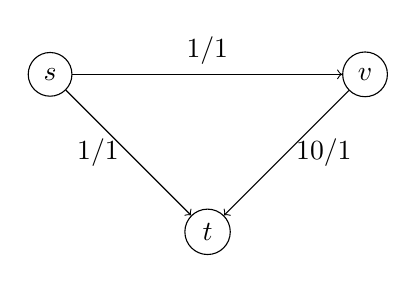
\begin{tikzpicture}
	\node[draw, circle] (S) at (0,2) {$s$};
	\node[draw, circle] (V) at (4,2) {$v$};
	\node[draw, circle] (T) at (2,0) {$t$};
	
	\path [->] (S) edge node[above] {$1/1$} (V);
	\path [->] (S) edge node[left] {$1/1$} (T);
	\path [->] (V) edge node[right] {$10/1$} (T);
	\end{tikzpicture}
	\caption{In der Abbildung ist ein Netzwerk mit Kantenbeschriftung $\tau_e / u_e$ zu erkennen.
		Man betrachte den dynamischen Nullfluss mit Zeithorizont $0$.
		Die Kanten $st$ und $sv$ sind aktiv, wohingegen die Kante $vt$ inaktiv ist.
		Dann ist der Fluss $x'$ mit $x_{sv}'=0$ und $x_{st}'=2$ nach \cite[Definition 6]{Koch2011} ein schmaler Fluss mit Zurücksetzen auf $\emptyset$ und Knotenbewertungen $l_s' = 1$, $l_v' = 0$ und $l_t' = 2$, aber für eine $\alpha$-Erweiterung ist $l_v(\theta) = \theta + 1 > 1 = l_v(0) + l_v' \theta$ für $\theta > 0$.} 
	\label{figure-labels}
\end{figure}